\documentclass{article}
\usepackage{enumitem}
\usepackage{graphicx}
\usepackage{grffile}
\usepackage{float}
\begin{document}
\title{%
 Deliverable 2\\
 \large An analysis and selection of software architecture, internal design\\
 \large and interface composition
}
\author{Epic Group}
\date{}
\maketitle

\section*{Introduction}
The purpose of this report is to clarify and justify the design components of 
CinemaScout, a web-based movie recommendation platform. The report will consist
of the following components:
\subsubsection*{Part 1}
\begin{enumerate}
\item \textbf{External Data Sources}: An enumeration over the third-party data
sources CinemaScout will access.
\item \textbf{Software Components}: A list of the major software components
that will be required for CinemaScout to function.
\item \textbf{Component Choices}: A list and justification of the choice of
software components for CinemaScout.
\item \textbf{Machine Requirements}: A justification of the machine requirements
of CinemaScout.
\item \textbf{Summary}: A summary of the entailments the aforementioned
software architecture decisions provide.
\end{enumerate}
\subsubsection*{Part 2}
\begin{enumerate}
\item \textbf{User Stories}: An updated list of user stories relating to the
previous report.
\item \textbf{Sequence Diagrams}: An interaction diagram for each use case
of CinemaScout as described in the user stories.
\end{enumerate}
\section{Software Architecture}
\subsection{External Data Sources}
CinemaScout is a movie aggregator which requires comprehensive movie 
related information to function.
Foremost, we require an encompassing and comprehensive list of all
movies to date. In addition, the user expects each movie to be listed alongisde 
its creation date, title and rating among other title specific information. 
This will require an API (application programming interface) which provides 
such data for all movies in the database of CinemaScout.\newline \newline
There exists no comprehensive API which singly provides all information 
CinemaScout requires. As a result, we are required to source data from multiple
external databases:
\begin{itemize}
\item \textbf{IMDb}: The Interactive Movie Database provides archive
snapshots of its comprehensive movie data sets. However, the data provided
is limited in detail as it only contains metadata for each movie in the IMDb
database. The dataset of IMDb is sufficient in providing a list of all movies,
although specific details such as rating and plot are not provided.
\item \textbf{OMDb}: The Open Movie Database is a RESTful web service
which provides comprehensive movie information for a singular, specific title. 
OMDb completes our data requirements, compensating for the lack of detail
provided by IMDb.
\end{itemize}
Most critically, the information provided by the database snapshots of IMDb
are a requisite of making a query to OMDb. As a result, the two external data
sources complement each other and complete our data sourcing requirements.
\subsection{Software Components}
In general, the components of CinemaScout may be split into two categories: 
server and client. The client category provides a medium for a user to invoke
CinemaScout functionality, while the server category consists of functionality 
which fulfills solicited requests made by the client category. To this effect,
the components of CinemaScout are interdependent and must be interoperable in
order to function.\newline\newline
\textbf{Client Components}
\begin{itemize}
\item \textbf{Web Browser}: A web browser which must support HTML5 (HyperText 
Markup Language), CSS (Cascading Style Sheets) and Javascript interpretation.
\item \textbf{Stylesheet}: A responsive and multi-platform CSS framework.
\end{itemize}
\textbf{Server Components}
\begin{itemize}
\item \textbf{Webserver}: A HTTP and REST web application framework.
\item \textbf{Database Manager}: Software capable of sorting and parsing
hundreds of thousands of database entries in real time as required by the
web server.
\item \textbf{Database Storage}: A software solution capable of saving hundreds
of thousands of database entries into long term storage.
\item \textbf{HTML Files}: A HTML-based UI allowing a user to perform actions
with the webserver through a web browser.
\item \textbf{Javascript Files}: Software to support the functionality of
HTML files, extending the usability of the web interface.
\item \textbf{Testing Framework}: Software capable of fulfilling the unit
test requirements of the project.
\end{itemize}
\subsection{Component Choices}
Due to the large volume of data utilised by CinemaScout, the performance of each
software component is critical in order to maintain a responsive user experience.
Therefore, the use of the C++ language for the webserver component has been
deemed as essential. Additionally, half of the development team is fluent with
the language, further justifying C++ as a viable language option for server.
This choice has influenced much of the other server components.\newline\newline
\textbf{Client Component Choices}
\begin{itemize}
\item \textbf{Web Browser}: Any browser which supports HTML5, CSS and Javascript
to any reasonable degree is compatible with the server.
\item \textbf{Stylesheet}: Bulma has been selected as a responsive, lightweight
and cross-platform CSS framework, enabling the website to function on mobile
and desktop devices without specific HTML implementation.
\end{itemize}
\textbf{Server Component Choices}
\begin{itemize}
\item \textbf{Webserver}: Pistache has been selected as it is a modern and
elegant, asynchronous HTTP and REST framework for C++.
\item \textbf{Database Manager}: The C++ standard library contains several
data structures and algorithms to accelerate server performance and reduce
code duplication. The database manager must be developed for CinemaScout
to function.
\item \textbf{Database Storage}: The C++ library RapidJSON has been selected
for database storage, as JSON is a lightweight and human readable solution,
aiding server performance and software complexity.
\item \textbf{HTML Files}: The layout of the website administered by HTML files
does not exist and must be developed from scratch.
\item \textbf{Javascript Files}: The functionality of the website, dependent
on the layout of the website, does not exist and must be developed from scratch.
\item \textbf{Testing Framework}: The C++ testing framework GoogleTest has
been selected as a modern solution for providing unit tests.
\end{itemize}
\subsection{Machine Requirements}
In order to maximise our target audience and minimise running costs, we have 
decided to enforce lax machine requirements for both the server and client
portions of the project. It is necessary that devices meet all of the following
criteria for CinemaScout to function correctly.\newline\newline
\textbf{Client}
\begin{itemize}
\item \textbf{Web Browser}: Any modern browser with Javascript and HTML5
support, along with the ability to store cookies.
\item \textbf{Internet Connection}: At least 1 MB/s download for images to load 
timely.
\item \textbf{Performance}: A device capable of meeting the previous criteria
to a reasonable degree.
\end{itemize}
\textbf{Server}
\begin{itemize}
\item \textbf{Operating System}: Any recent Linux derivative.
\item \textbf{Performance}: Dependent on website traffic. CPU speed and memory
bandwidth and size should be maximised for faster runtime performance and user
session persistence. Low disk speed requirements as it is rarely used aside
from during initialisation.
\item \textbf{Compiler}: A compiler with C++20 support. Capable of building and
linking with Boost, libCurl, Pistache, GoogleTest while building with CMake.
\item \textbf{Internet Connection}: At least 10 MB/s upload and download to 
anticipate rapid surges of website traffic.
\end{itemize}
\subsection{Summary}
The use of C++ as the programming language for the server alongside the native
C++ libraries  RapidJSON, Pistache, libCurl as well as the C++ standard library
will allow the server to deliver accurate movie suggestions in real time for a
responsive user experience. The use of JSON as a data storage format will 
prevent unnecessary database queries, decreasing server boot time and
individual request response time.
\newline\newline
Bulma as a CSS framework will enable the website to
function responsively on both mobile and desktop user browsers. Finally,
selecting both OMDb and IMDb as external data sources will enable the user
to receive relevant and comprehensive movie information via the frontend.
\section{Initial Software Design}
\subsection{User Stories}
\begin{itemize}
\item \textbf{User Story}: As an avid film watcher, I want to receive 
tailored, specific recommendations relevant to me.
\newline\textbf{Sequence Diagram}: See Figure 1.
\item \textbf{User Story}: As someone who enjoys multiple movie genres, I want
to receive recommendations which are not based on my previous viewing sessions.
\newline\textbf{Sequence Diagram}: See Figure 1.
\item \textbf{User Story}: As a power user, I wish to be able to receive many 
movie recommendations over a short period of time.
\newline\textbf{Sequence Diagram}: See Figure 1.
\item \textbf{User Story}: As a first time website visitor, I wish to be able 
to perform a search without offering my credentials and other personal
information to first generate an account.
\newline\textbf{Sequence Diagram}: See Figure 1.
\item \textbf{User Story}: As a user of the service, I wish to be able to use 
the service in its full capability without malicious content from ever 
corrupting my movie suggestions.
\newline\textbf{Sequence Diagram}: See Figure 1.
\item \textbf{User Story}: As a user of the service, I do not wish to receive
recommendations based on corporate interests or monetary influence.
\newline\textbf{Sequence Diagram}: See Figure 1.
\item \textbf{User Story}: As a returning user of the service, I wish to be able
to view my recommendations and come back to my search results later.
\newline\textbf{Sequence Diagram}: See Figure 2.
\item \textbf{User Story}: As a user of CinemaScout who likes to watch trailers
before the film, I wish to be able to view trailers for my recommendations
in the CinemaScout website.
\newline\textbf{Sequence Diagram}: See Figure 3.
\item \textbf{User Story}: As a user of CinemaScout who wishes to view
the results of the search offline, I want to be able to download the search
results in a readable format for offline use.
\newline\textbf{Sequence Diagram}: See Figure 4.
\item \textbf{User Story}: As a user of CinemaScout who wants to print out my
results, I wish to be able to print out a formatted version of the results page
tailored for readability on an A4 page.
\newline\textbf{Sequence Diagram}: See Figure 5.
\end{itemize}
\subsection{Sequence Diagrams}
\begin{figure}[H]
\includegraphics[width=\columnwidth]{res/sequence_diagram.png}
\caption{Typical CinemaScout Use Case}
\end{figure}

\begin{figure}[H]
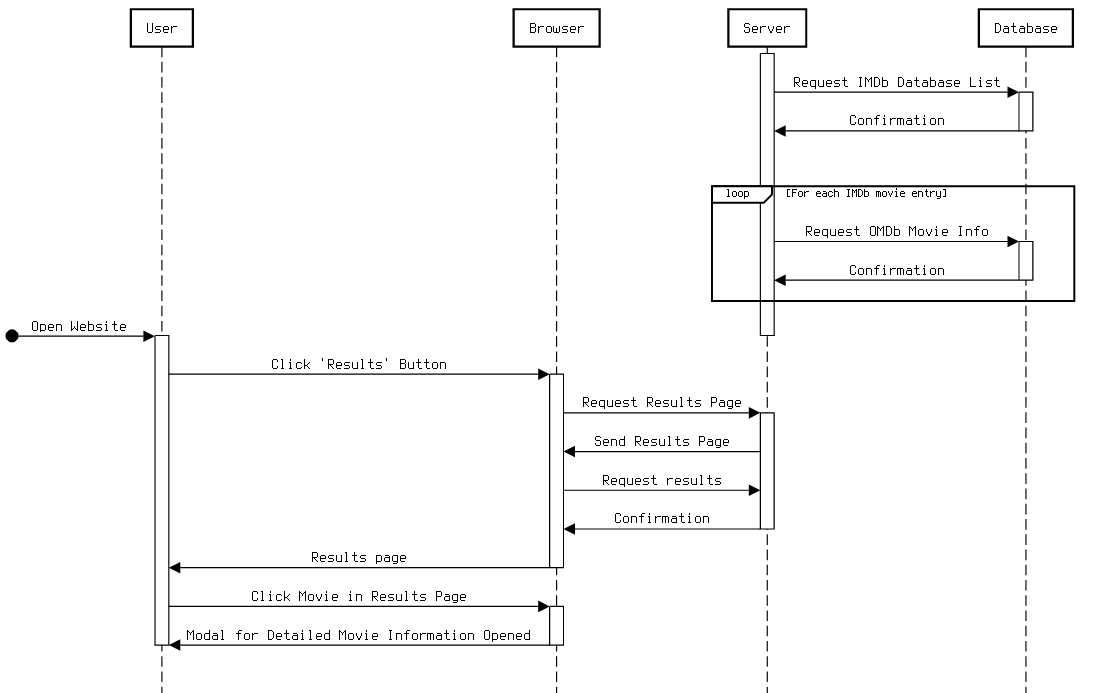
\includegraphics[width=\columnwidth]{res/sequence_diagram2.png}
\caption{Previous Results Use Case}
\end{figure}

\begin{figure}[H]
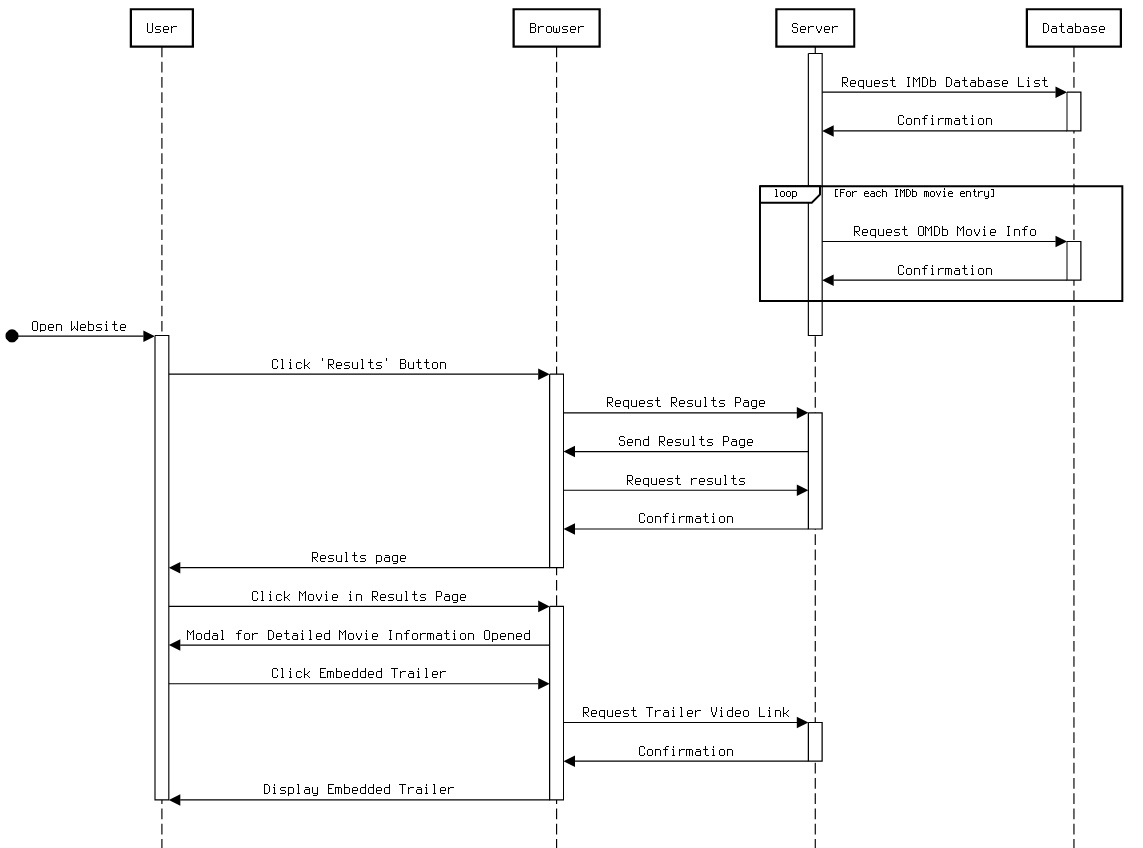
\includegraphics[width=\columnwidth]{res/sequence_diagram3.png}
\caption{Embedded Trailer Use Case}
\end{figure}

\begin{figure}[]
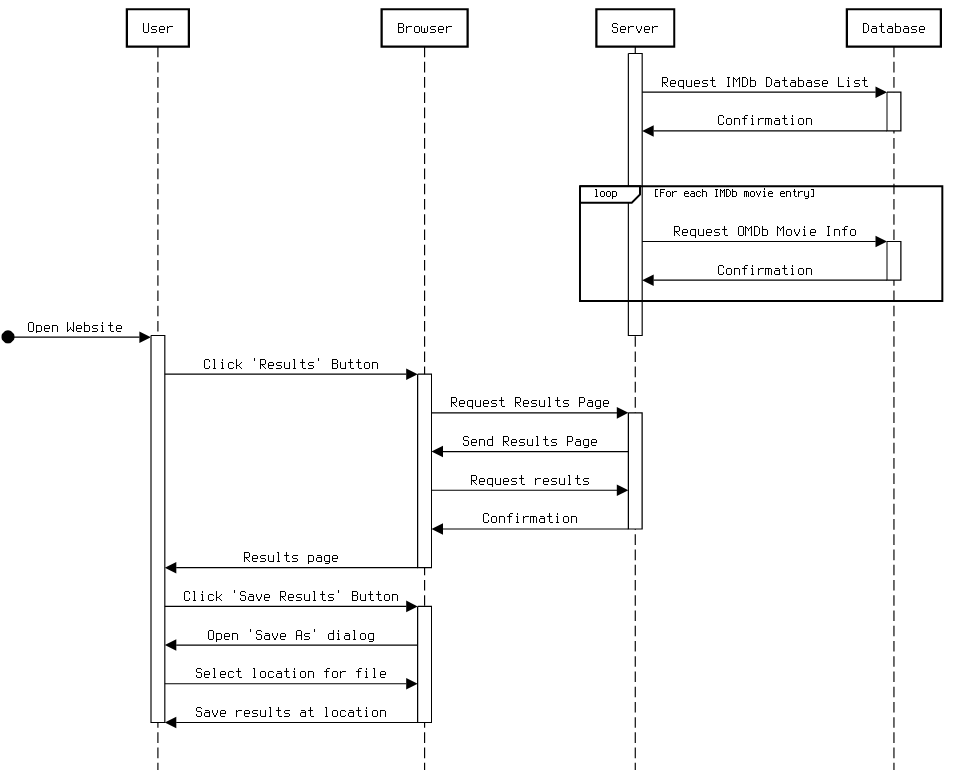
\includegraphics[width=\columnwidth]{res/sequence_diagram4.png}
\caption{Save to File Use Case}
\end{figure}


\begin{figure}[]
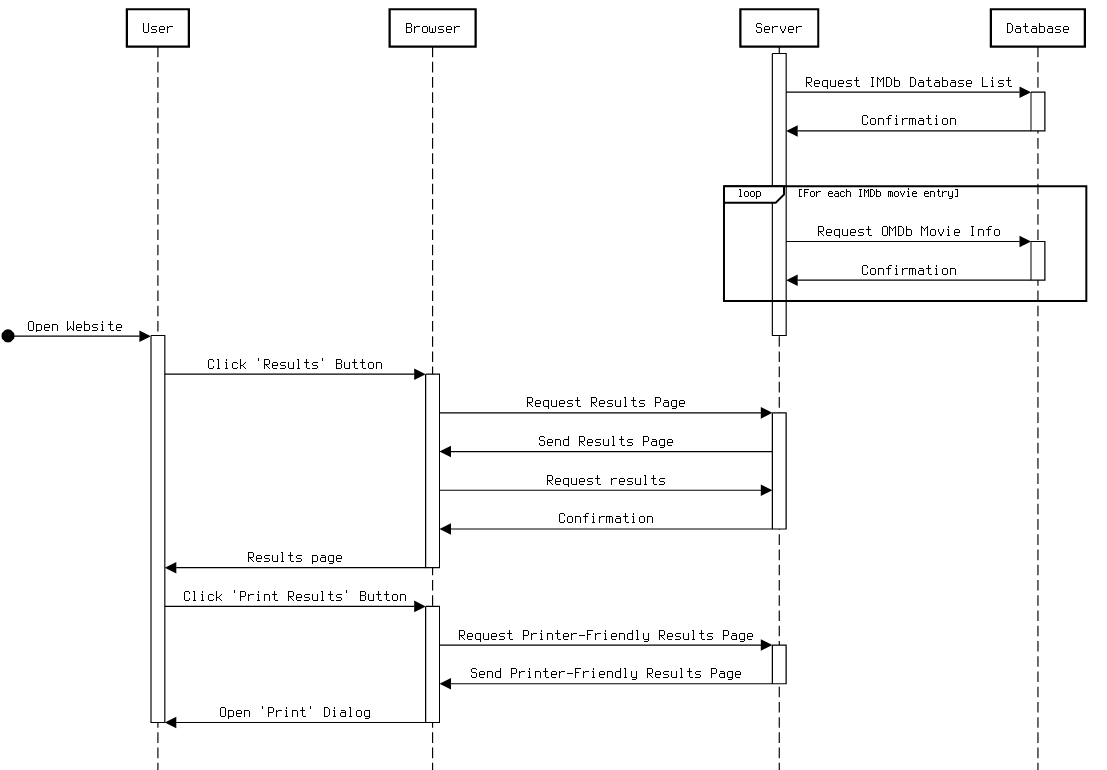
\includegraphics[width=\columnwidth]{res/sequence_diagram5.png}
\caption{Print Results Use Case}
\end{figure}

\end{document}
